% Generated from tex/chapters/ch04/08_構築技術.tex for the SWEBOK structure tree
\subsubsection{実行可能モデル}

実行可能モデルとは、特定のプログラミング言語や実装構造の詳細から離れて、実行できる形で振る舞いを表すモデルである。実行可能 UML などが例である。

モデル駆動アーキテクチャでは、プラットフォーム非依存モデルとプラットフォーム固有モデルを区別する。プラットフォーム非依存モデルは、実装環境に依存しない解決策を表す。プラットフォーム固有モデルは、特定のハードウェアやソフトウェア環境の詳細を含む。変換器は、非依存モデルとプラットフォーム情報を組み合わせ、実装を生成する。

\begin{figure}[htbp]
\centering
\IfFileExists{assets/generated_figures/ch04/fig-ch04-10.png}{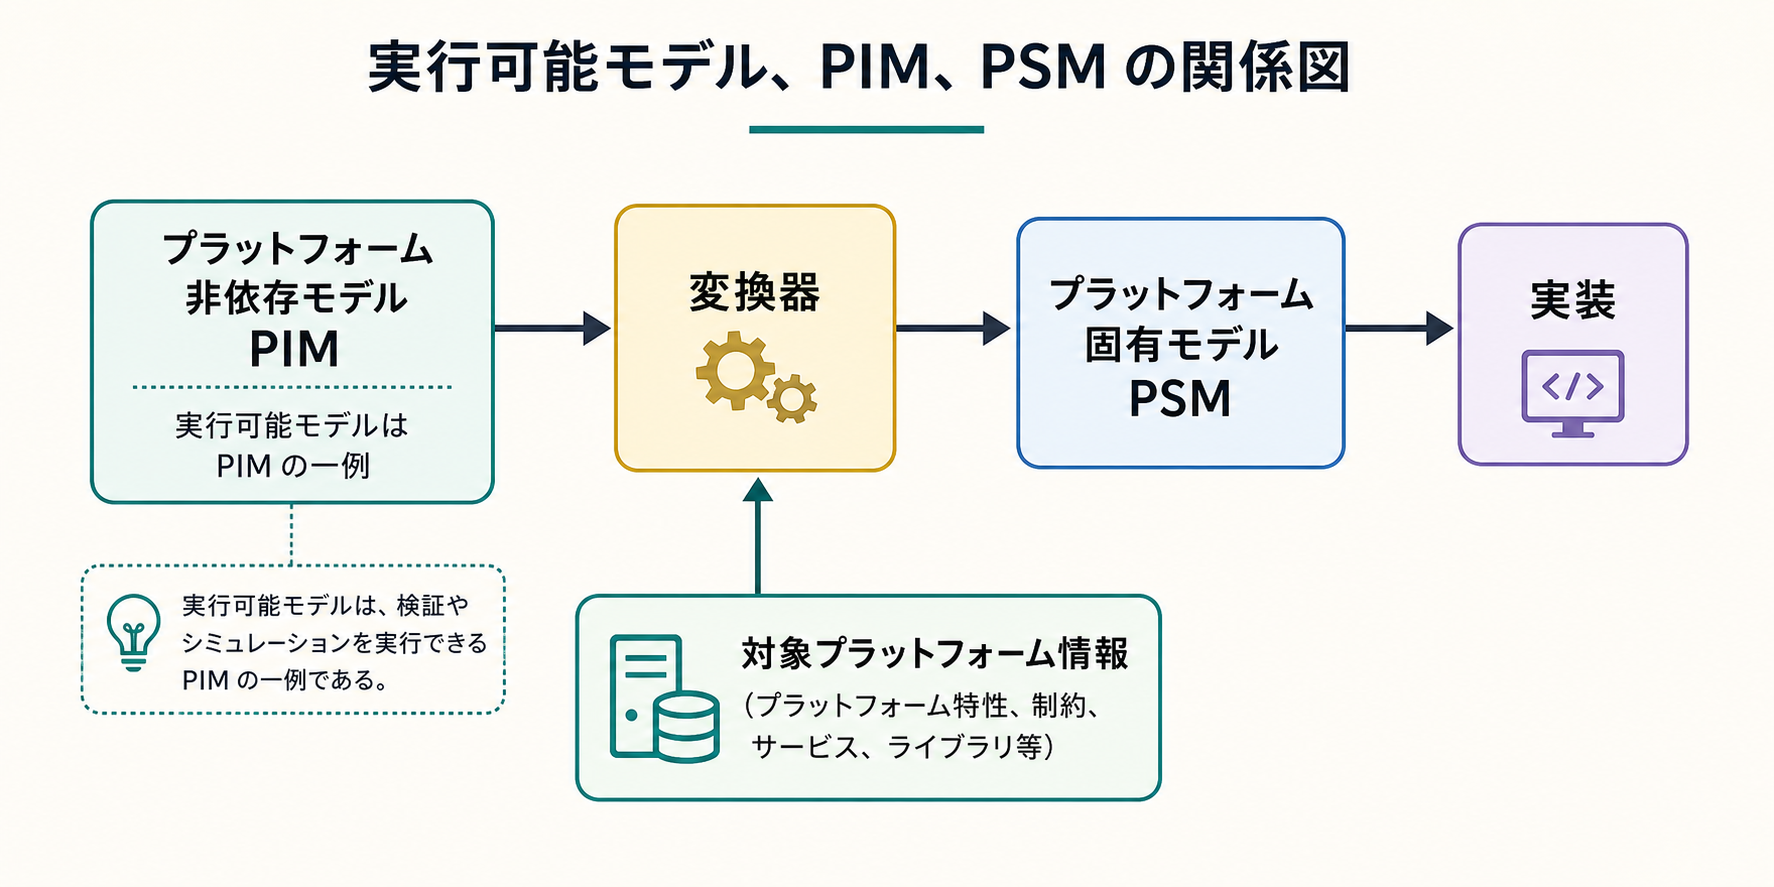
\includegraphics[width=0.96\linewidth]{assets/generated_figures/ch04/fig-ch04-10.png}}{\fbox{\parbox[c][48mm][c]{0.9\linewidth}{\centering 画像生成待ち\\実行可能モデル、PIM、PSM の関係図}}}
\caption{実行可能モデル、PIM、PSM の関係図}
\label{fig:ch04-10}
\end{figure}
